\section{Numerical Experiments}
\label{sec:experiments}


\subsection{Empirical Validation of DGSim}
\label{sec:experiments:validation}
\begin{table}
\caption{DGSim parameters for load balance comparison.
%The NUMA domains corresponds NUMA domains per node.
%Worker threads corresponds to worker threads per NUMA domain.
%$R-K$ stages is the total number of Runge-Kutta stages simulated.
%$p$ is the polynomial order of the DG method.
%The rebalance frequency corresponds to the delay between which tiles send messages to the world model. $\alpha$ and $\beta$ are the parameters in the cost model $C(N) = \alpha N/N_{\text{total}} + \beta$.
}
\label{tab:lbc:machine}
\centering
{ \scriptsize
\begin{tabular}{|l|c|l|c|}
\hline
\multicolumn{2}{|c|}{Machine} & \multicolumn{2}{|c|}{DGSWEM} \\
\hline
NUMA domains/node   & 2       & Runge-Kutta Stages     & 273600 \\
Threads/NUMA domain & 12      & Polynomial order ($p$) & 2      \\ 
CPU clock-speed & 2.4 GHz & Tiles/worker thread    & 4      \\
\hline
\multicolumn{2}{|c|}{Asynchronous Diffusion} & \multicolumn{2}{|c|}{Semi-Static} \\
\hline
Rebalance Frequency &  $40\,\mathrm{ms}$  & Rebalance Frequency & $5\,\mathrm{s}$ \\
$\alpha$ & 1 & &  \\
$\beta$ & 2 & & \\
\hline
\end{tabular}
}
\end{table}

To ensure that our simulator is accurate, we compared the DGSim execution times for the Storm36 synthetic hurricane simulation to a skeletonized version of DGSWEM run on NERSC's Edison.  The skeletonized DGSWEM implements the programming model outlined in Section~\ref{sec:dgsim}. Inter-process communication is achieved through one-sided asynchronous remote procedure calls using UPC++~\cite{Bachan2017}, and tasks are executed using a dataflow execution model with a master-worker thread organization.
One feature not implemented in the skeletonized DGSWEM is the AGAS layer. However, for the statically balanced problems considered for this validation, AGAS overhead is negligible due to caching of neighbors' ranks.
By burning identical worker thread execution times, the validation examines whether the messaging and threading overhead models as described in Section~\ref{sec:compute-cost-model} are reasonable.
%, implemented using the programming model described in Section~\ref{sec:dgsim}. 
The parallel efficiencies for the two simulations are shown in Figure~\ref{fig:cal:validation}. Differences in execution times between the simulation and the skeletonized DGSWEM application do not exceed 7\% of the runtime. Furthermore, the DGSim execution time was slower than the DGSWEM execution time for all simulations, reflecting the conservative design of our cost models.  These validation results demonstrate that despite our relatively simple network model, DGSim predicts execution times for this particular hurricane simulation with accuracies comparable to more sophisticated approaches, e.g. \cite{Stanisic2015,Jain2016}.

\begin{figure}
  \centering
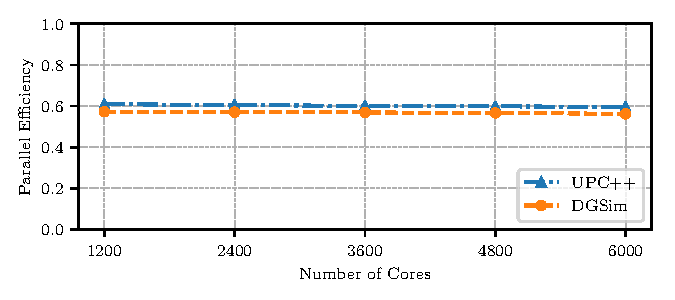
\includegraphics{{load_balancing/images/hurricane_validation_p2}.pdf}
\caption{Comparison between the parallel efficiency of the simulated performance (DGSim) and the skeletonized application code (DGSWEM) on NERSC's Edison supercomputer for 1200 to 6000 cores for the Storm36 hurricane using Machine and DGSWEM parameters as outlined in Table~\ref{tab:lbc:machine}. Each configuration was run five times. The standard deviations for a given core count were each below 1\%.}
\label{fig:cal:validation}
\end{figure}

\subsection{Load Balance Comparison}
In order to compare the load balancing algorithms outlined in Section \ref{sec:balancers}, we compare performance for the hurricane used in the previous subsection using a fixed machine and algorithmic configuration outlined in Table \ref{tab:lbc:machine}. The load balancer parameters are based on parameter sweeps done at 1200 and 3600 cores.

\begin{figure*}
\centering
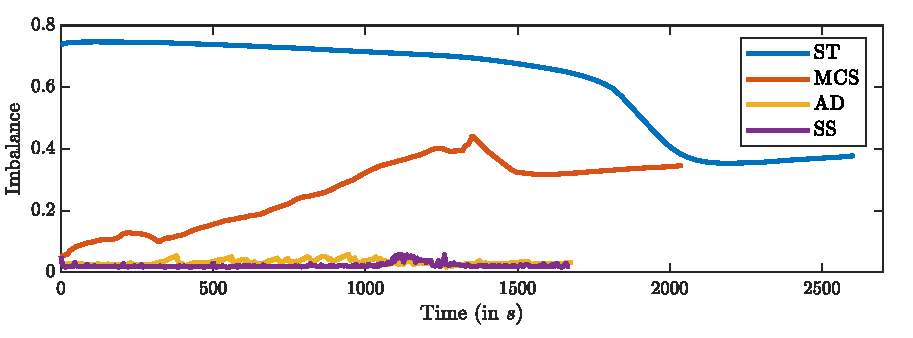
\includegraphics{{load_balancing/images/imbalance}.pdf}
\caption{Load imbalance for Storm 36 using 1200 cores with the configuration outlined in Table \ref{tab:lbc:machine}. The following load balancing strategies were evaluated: static (ST), multi-constraint static (MCS), asynchronous diffusion (AD), and semi-static (SS).}
\label{fig:lbc:imb}
\end{figure*}
%\clearpage
\begin{sidewaystable}
  \centering
  \caption{Performance of load balancers for Storm36}
  \label{tab:sss:res}
	\begin{threeparttable}
	{\footnotesize
	%Generated with make_tables.py
%Do not edit this file directly
%Rather edit make_tables.py
\begin{tabular}{|c||c|c|c|c|c|c|c|c|c|c|c|c|c|}
\hline
& \multicolumn{1}{|c|}{Static} & \multicolumn{2}{|c|}{Multi-constraint static} & \multicolumn{5}{|c|}{Asynchronous diffusion} & \multicolumn{5}{|c|}{Semi-static} \\
\hline
Cores & $T_{\text{ST}}$ & $T_{\text{MC}}$ & $S_{ST}$ & $T_{\text{AD}}$ & TM & $\sigma_{TM}$ & $S_{ST}$ & $S_{MC}$ & $T_{\text{SS}}$ & TM & $\sigma_{TM}$ & $S_{ST}$ & $S_{MC}$ \\
\hline
1200 & 2,613 & 2,048 & 1.28 & 1,686 & 3,654 & 145 & 1.55 & 1.21 & 1,675 & 723,109 & 2,325 & 1.56 & 1.22 \\
\hline
2400 & 1,310 & 1,058 & 1.24 & 849 & 9,532 & 189 & 1.54 & 1.25 & 856 & 681,654 & 557 & 1.53 & 1.24 \\
\hline
3600 & 876 & 698 & 1.26 & 571 & 16,614 & 319 & 1.53 & 1.22 & 585 & 641,950 & 568 & 1.50 & 1.19 \\
\hline
4800 & 659 & 553 & 1.19 & 431 & 24,402 & 319 & 1.53 & 1.28 & 452 & 593,709 & 3,932 & 1.46 & 1.22 \\
\hline
6000 & 528 & 444 & 1.19 & 348 & 36,955 & 761 & 1.52 & 1.28 & 373 & 574,109 & 1,255 & 1.41 & 1.19 \\
\hline
\end{tabular}

	}
	\begin{tablenotes}[para,flushleft]
{\bf Note:} All times are reported in seconds. For each case, 5 runs were performed. The standard deviation of all execution times was found to be below 2\% of the mean. $T$ corresponds to the execution time in seconds. TM refers to the number of relocated tiles. The speed-up $S_X$ is the speed-up of the simulation relative to strategy $X$ at the given core count. Due to non-determinism in our simulation, we've reported standard deviations of tiles moved $\sigma_{TM}$ for a sample size of 5.
\end{tablenotes}
	\end{threeparttable}
\end{sidewaystable}

%\begin{table}[t!]
%\small
%\centering
%\input{images/lb_comparison_table_p2_tpt4}
%\caption{Run-times $T$, in seconds, for the load balancing strategies. The presented speed-ups $S$ are with respect to the static run-time. $TM$ represents the numbers of tiles moved. The non-deterministic nature of the simulation causes variance in the results. We have shown the respective standard deviations $\sigma$ for a sample size of 5. The standard deviations of all the timing data is within 1\%.}
%\label{tab:lbc:speedup}
%\vspace{-7mm}
%\end{table}
%discuss advantage of going to static1

To quantify the quality of our load balancing algorithms, we use two performance metrics: the
\emph{compute intensity}, which is defined for a given rank as the fraction of time spent computing at a given instant in the simulation, and the \emph{imbalance}, which is defined as
\begin{equation*}
I = \frac{ \max T - \overline{T}}{\overline{T}},
\end{equation*}
where $\max T$ is maximum load on a given rank and $\overline{T}$ is the average load across the system. The combined performance results are shown in Figure~\ref{fig:lbc:imb} and the elapsed times and speed-ups in Table \ref{tab:sss:res}.

\begin{figure*}
    \centering
    \subfloat[][Static\label{fig:ci:st}]{
        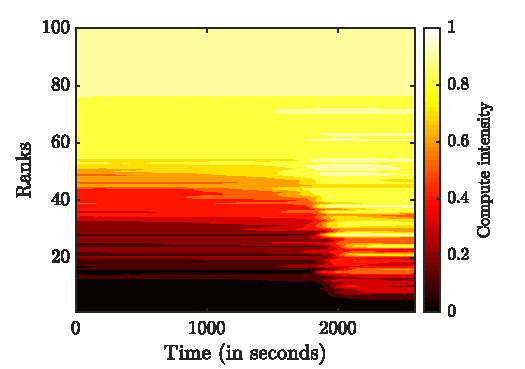
\includegraphics[width=0.44\textwidth]{{load_balancing/images/st_comput_int}.pdf}
    }
\quad
    \subfloat[][Multi-constraint static\label{fig:ci:mcs}]{
        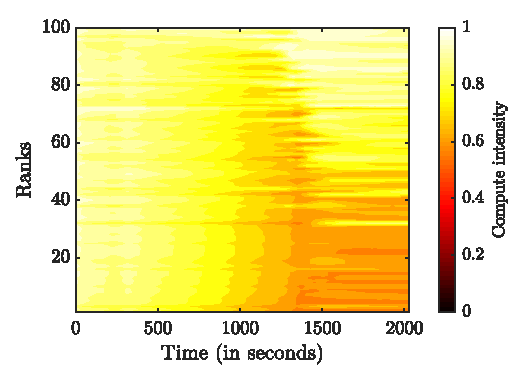
\includegraphics[width=0.44\textwidth]{{load_balancing/images/mcs_comput_int}.pdf}
    }
\\
    \subfloat[][Asynchronous diffusion\label{fig:ci:ad}]{
        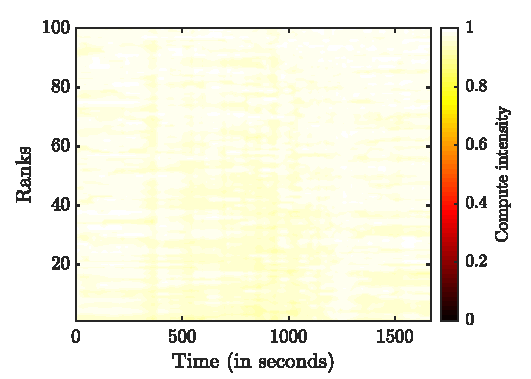
\includegraphics[width=0.44\textwidth]{{load_balancing/images/ad2_comput_int}.pdf}
    }
\quad
    \subfloat[][Semi-static\label{fig:ci:ss}]{
        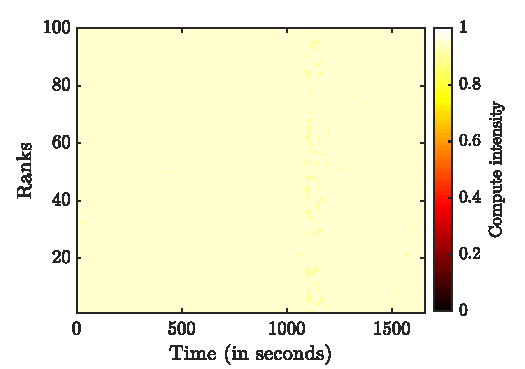
\includegraphics[width=0.44\textwidth]{{load_balancing/images/ss_comput_int}.pdf}
    }
    \caption{Compute intensities of the various load balancing strategies for a 1200 core simulation. For clarity, the ranks have been sorted according to average compute intensity.}
    \label{fig:ci}
\end{figure*}

Since the traditional static load balancing approach solely distributes tiles to ranks to satisfy the memory constraint, it is expected that the static curve in Figure \ref{fig:lbc:imb} has a high imbalance. This is reflected in Figure \ref{fig:ci:st}, where roughly half the ranks are underutilized until the storm inundates the coast. This load profile is consistent with the ~60\% parallel efficiency observed in Figure \ref{fig:cal:validation}.
The multi-constraint static load balancer takes load as well as memory into account. This results in much better load balance until the hurricane makes landfall. Once this happens, the dynamic nature of the computational load causes a strong increase in imbalance and a corresponding decrease in computational intensity. Since the majority of the time DGSWEM simulates is prior to landfall, the multi-constraint static mesh partitioning achieves a speed-up of 1.28 versus the original static partitioning.

Both the asynchronous diffusion and semi-static load balancers are very effective at reducing load imbalance. The compute intensities shown in Figure~\ref{fig:ci:ss} and \ref{fig:ci:ad} illustrate the ranks are being well utilized throughout the simulation. With roughly equal execution times, both load balancers achieve 96\% of the ideal parallel efficiency. 
While the semi-static strategy migrates significantly more tiles than asynchronous diffusion, we have observed a small dependence of execution time in DGSIM on tiles moved.
% We have examined means to reduce the number of times.
AGAS's ability to overlap computation and tile migration minimizes resource starvation. Furthermore, the execution time is mainly determined by the simulation's critical path. Thus migrating tiles not on the critical path will not impact execution time.


\subsection{Strong Scaling Study}
To demonstrate that these algorithms are scalable for operationally-relevant core counts, we present a strong scaling study for up to 6000 cores. 
%Describe simulation
To obtain an understanding of the quality of the load balancers relative to achievable performance, we define the parallel efficiency $E$ for load balancer $LB$ as $E_{LB} = \frac{ T^*}{n_c T_{LB}}$ where $T^*$ is the serial execution time, $n_c$ is the core count, and $T_{LB}$ is the execution time at a given core count. As the master threads do not compute tasks themselves, the best attainable parallel efficiency is 91.7\% = 11/12.

Using the parameters Table \ref{tab:lbc:machine}, the parallel efficiencies for the four partitioning strategies are shown in Figure~\ref{fig:sss:res}. Note that by fixing  tiles per worker thread, the task granularity decreases as we scale out to higher core counts.
Firstly, we note that the code scales well: the static partitioning strategy loses less than 1\% parallel efficiency across the range of core counts. The execution time here should be similar to that of a fully wetted mesh, and demonstrates the parallelizability of the DG method. Next, the multi-constraint static partitioner experiences a slight degradation in performance; $E^{MC}_{6000}/E^{MC}_{1200} = 92.1 \%$. As the number of cores increases each NUMA domain is assigned a smaller fraction of the mesh. Scaling out, the imbalance becomes more sensitive to local inundation, causing degradation of the strong scaling performance.

The semi-static load balancer also loses efficiency at scale with $E^{SS}_{6000}/E^{SS}_{1200}=89.6\%$. Since the rebalance frequency is fixed by the trellis approach, as we scaled out to larger core counts, the number of times the balancer is called decreases. Furthermore, the cost of repartitioning the tile graph increases: at 6000 cores, the METIS calls take approximately 3.7 seconds. We suspect that the performance degradation is due to both the faster rate that imbalance is introduced, as well as a mismatch between the load balance used to compute the repartitioning and the load balance at the time when the AGAS migrates get issued. %\todo{See if noburn results help explain things better}
 Ultimately, the performance appears to remain robust, with the semi-static partitioner maintaining a speed-up of 1.19 over the multi-constraint static partitioner at 6000 cores.

The asynchronous diffusion load balancing scales the best with $E^{AD}_{6000}/E^{AD}_{1200} = 96.9\%$. Since the cost of rebalancing is entirely local, the computational complexity of load balancing decisions does not grow with the number of cores. Furthermore, since the rebalancing frequency is roughly two orders of magnitude higher than the semi-static rebalancing frequency, the asynchronous diffusion approach does not struggle with increased irregularity due to higher core counts. A common problem with strong scaling of diffusion-based algorithms is the persistence of small gradients. Even with finer tiles at large core counts, as the rank graph grows, the maximum allowable imbalance grows as well. This did not appear to be a problem here. However, we do not claim that this approach would work equally well for other applications. Ultimately, the asynchronous diffusion worked very well providing a speed-up of 1.28 over the multi-constraint static partitioning strategy at 6000 cores, and achieved 93.7\% of the maximum attainable speed-up.

\begin{figure}
\centering
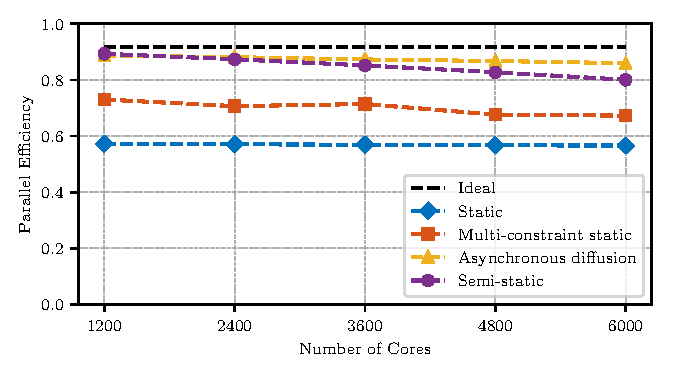
\includegraphics{{load_balancing/images/strong_scaling_p2_tpt4_figure}.pdf}
\caption{Parallel efficiency of the various load balancing strategies on Edison for 1200 to 6000 cores.}
\label{fig:sss:res}
\end{figure}

